\begin{figure}[htbp]
\centering 
    \subfloat[Frontal view. t = 150 s.]{
	  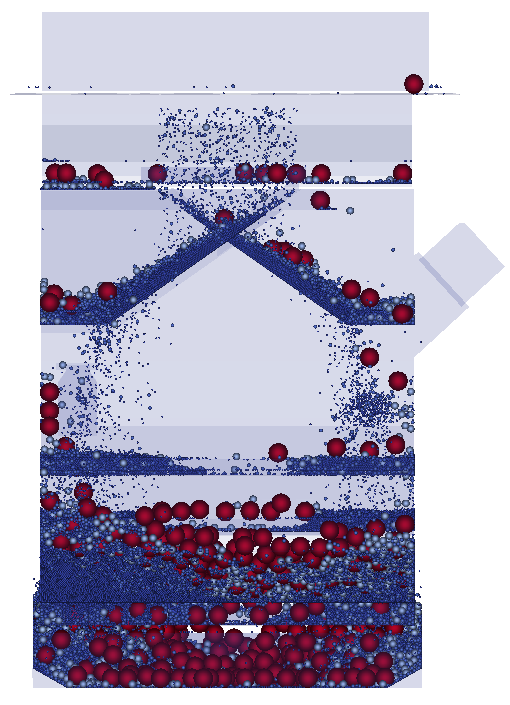
\includegraphics[width=.25\columnwidth]{images/303frontalLayout150}
	  \label{fig:303frontalLayout150}  }
 \quad
   \subfloat[Lateral view. t = 150 s.]{
	  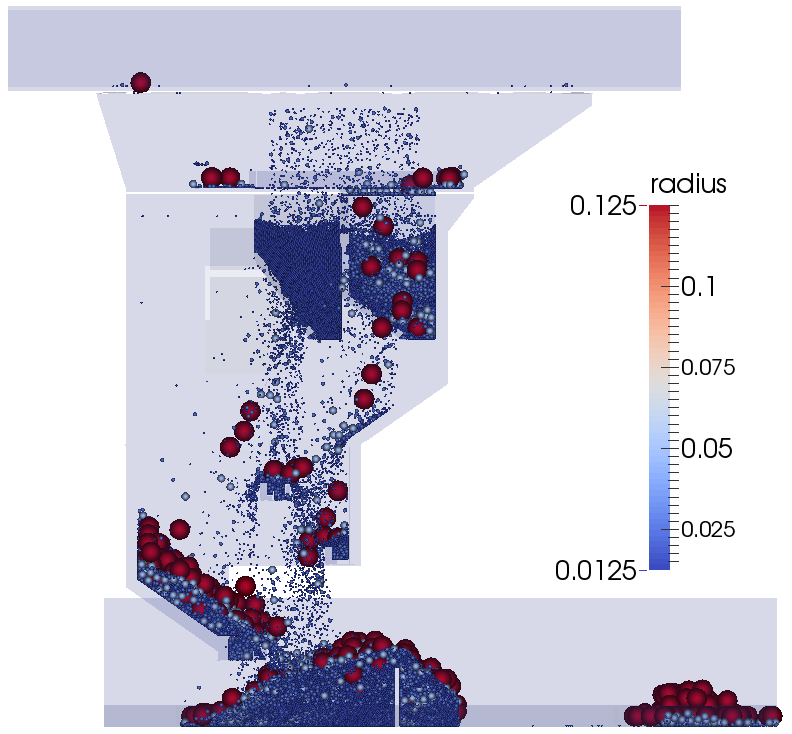
\includegraphics[width=.37\columnwidth]{images/305lateralLayout150}
	  \label{fig:305lateralLayout150}  }
  \\
  \subfloat[Frontal view. t = 200 s.]{
	  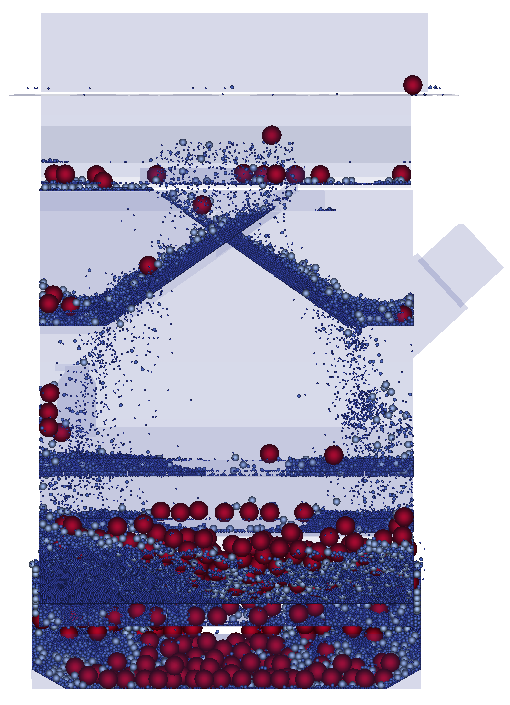
\includegraphics[width=.25\columnwidth]{images/304frontalLayout200}
	  \label{fig:304frontalLayout200}  }
  \quad 
  \subfloat[Lateral view. t = 200 s.]{
	  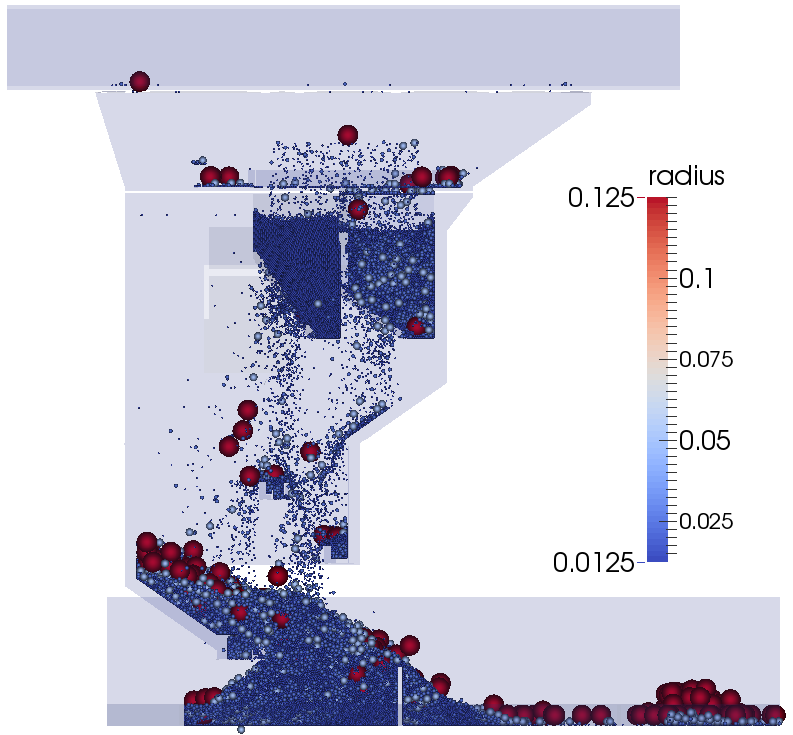
\includegraphics[width=.37\columnwidth]{images/306lateralLayout200}
	  \label{fig:306lateralLayout200}  }
  \\
  \subfloat[Frontal view. t = 250 s.]{
	  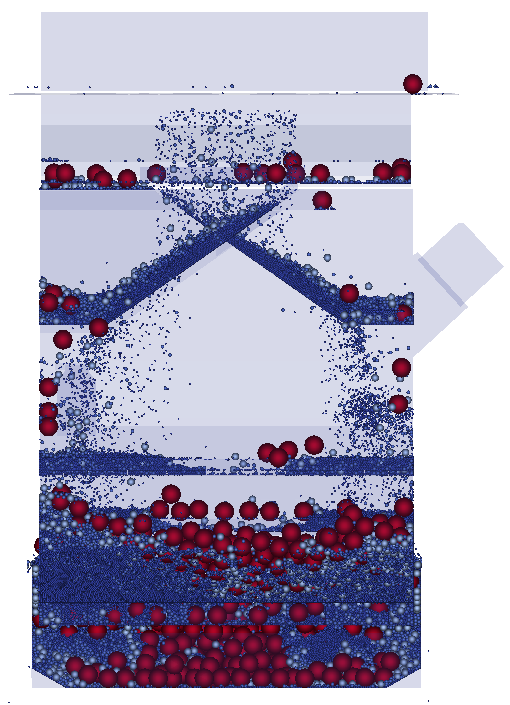
\includegraphics[width=.25\columnwidth]{images/301frontalLayout250}
	  \label{fig:301frontalLayout250}}
    \quad	  
  \subfloat[Lateral view. t = 250 s.]{
	  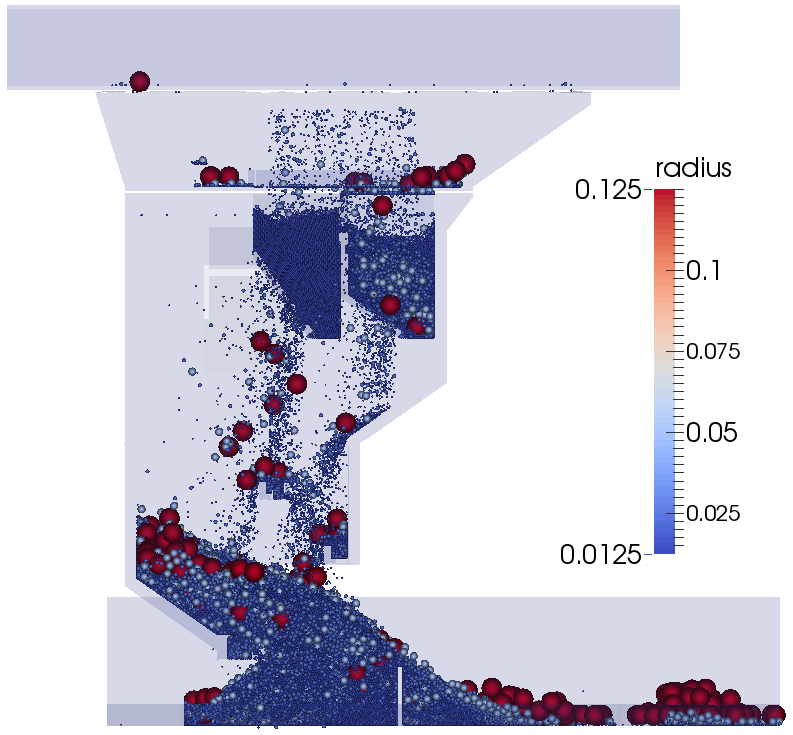
\includegraphics[width=.37\columnwidth]{images/302lateralLayout250}
	  \label{fig:302lateralLayout250}  }  
  \\
  \caption[Simulation screenshots]{Sinter chute simulation screenshots.
  Particles are tracked to ascertain the segregation behaviour.}
  \label{fig:097particlespositions}
\end{figure}